\documentclass[a4paper,12pt]{article}

\usepackage[utf8]{inputenc}
\usepackage[T1]{fontenc}
\usepackage[french]{babel}
\usepackage{titling}
\usepackage{geometry}
\usepackage{graphicx}
\usepackage{listings}
\usepackage{xcolor}
\usepackage{amsmath}


\geometry{a4paper, margin=1in}

\title{Mini-projet : Estimation d'aires par la methode de Monte Carlo}
\author{Alexandre Bertho}
\date{\today}

\lstset{
  language=R,
  basicstyle=\ttfamily\small,
  keywordstyle=\color{blue!50!black},
  commentstyle=\color{green!50!black},
  stringstyle=\color{red!50!black},
  breaklines=true,
  breakatwhitespace=false,
  tabsize=2,
  backgroundcolor=\color{white},
  frame=single,
  frameround=fttt,
  framesep=3pt,
  showspaces=false, % Supprime les caractères non-ASCII
  showstringspaces=false, % Supprime les caractères non-ASCII dans les chaînes de caractères
  literate = % Resout problème utf 8 crédit :(https://www.mathweb.fr/euclide/2020/07/09/latex-et-listings-en-utf8/)
  {é}{{\'e}}{1}% 
  {è}{{\`e}}{1}%
  {à}{{\`a}}{1}%
  {â}{{\^a}}{1}%%%
  {ç}{{\c{c}}}{1}%
  {œ}{{\oe}}{1}%
  {ù}{{\`u}}{1}%
  {É}{{\'E}}{1}%
  {È}{{\`E}}{1}%
  {À}{{\`A}}{1}%
  {Ç}{{\c{C}}}{1}%
  {Œ}{{\OE}}{1}%
  {Ê}{{\^E}}{1}%
  {ê}{{\^e}}{1}%
  {î}{{\^i}}{1}%
  {ï}{{\"i}}{1}%%%
  {ô}{{\^o}}{1}%
  {û}{{\^u}}{1}
}

\begin{document}

\begin{titlepage}
    \begin{center}
        \vspace*{1cm}
        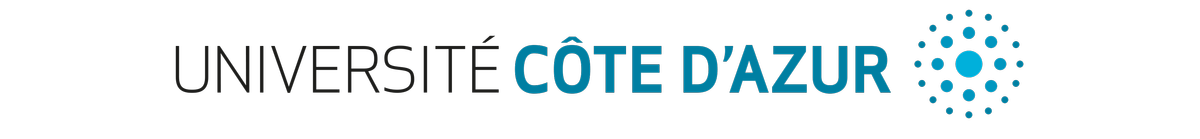
\includegraphics[width=1\textwidth]{logo-univ.png}
        
        \textbf{\Large Algo \& Prog avec R}
        
        \vspace{0.5cm}
        \theauthor

        \vspace{1.5cm}
        \textbf{\Huge \thetitle}
        
        \vfill
        
        \large 
        \thedate
        
    \end{center}
\end{titlepage}

\section{Méthode de Monte Carlo pour approximer $\pi$}

\subsection{Estimation de $\pi$}

\subsubsection{Estimation de $\frac{\pi}{4}$}

L'aire totale du disque de rayon \( R = 1 \) est :

\[
\text{Aire du disque} = \pi R^2 = \pi
\]

L'aire du quart de disque est donc :

\[
\sigma = \frac{\pi R^2}{4} = \frac{\pi}{4}
\]

L'aire du carré unitaire qui contient ce quart de disque est :

\[
S = R^2 = 1
\]

La probabilité qu'un point \( M \) appartienne à ce quart de disque est le rapport de l'aire du quart de disque à l'aire du carré :

\[
P = \frac{\text{Aire du quart de disque}}{\text{Aire du carré}} = \frac{\sigma}{S} = \frac{\frac{\pi R^2}{4}}{R^2} = \frac{\frac{\pi}{4}}{1} \approx \frac{\pi}{4}
\]

\subsubsection{Application avec R}

Premirement on veut déterminer si un point de coordonnées ($x$, $y$) appartient à un cercle de centre (0, 0) et de rayon 1.
\\[1\baselineskip]
Un point ($x$, $y$) appartient au cercle si la distance entre ce point et le centre du cercle est inférieure ou égale au rayon $R$. Cette distance est calculée à l'aide de la formule de la distance :
\[
\sqrt{(x - a)^2 + (y - b)^2} \leq R
\]
Dans notre cas, $a = 0$ et $b = 0$, nous mettons au carré les deux côtés pour éviter de calculer la racine carrée  :
\[
x^2 + y^2 \leq R^2
\]
Finalemnt, un point ($x$, $y$) appartient au cercle si :
\[
x^2 + y^2 \leq 1
\]

\newpage

Voici une fonction R qui permet d'estimer $\pi$ en utilisant la méthode de Monte Carlo :

\begin{lstlisting}
mc.pi <- function(n) {
  # Génère n coordonnées x et y aléatoires uniformément dans [0, 1]
  x <- runif(n, 0, 1)
  y <- runif(n, 0, 1)
  
  # Compte le nombre de points à l'intérieur du quart de cercle de rayon 1
  # et estime Pi à partir de la proportion
  estimation_pi <- 4 * (sum(x^2 + y^2 <= 1) / n)
  
  return(estimation_pi) 
}
\end{lstlisting}

\subsection{Simulations avec \texttt{n=10**j, pour j=1:p} }


\begin{lstlisting}
t <- 50  # Nombre d'estimations par colonne
p <- 7   # Nombre de colonnes

# Initialiser la matrice PIE
PIE <- matrix(0, nrow = t, ncol = p)

# Remplir la matrice avec des estimations de pi
for (j in 1:p) {
    n <- 10^j  # Calculer n comme 10 à la puissance j
    for (i in 1:t) {
        PIE[i, j] <- mc.pi(n)  # Estimer pi et remplir la matrice
    }
}
  \end{lstlisting}

\end{document}